\section{Lorentztransformatie}
%%%%%%%%
%pretest\subsection{Lorentz-invariantie}
%pretestGa m.b.v. de Lorentztransformatie na dat formule 3.3 op blz. 11 van de 
%pretestsyllabus klopt.
%pretest
%pretest%%%%%%%%%%%
%pretest\subsection{Gamma}
%pretestGa na dat de vergelijking $a = \frac{1}{\sqrt{1 - \frac{v^{2}}{c^{2}}}}$
%pretestop blz. 13 van de syllabus correct is. 

%%%%%%%%%%%
\subsection{Inverse Lorentztransformatie}

% \begin{figure} [h]
% \begin{center}
% \mbox{\epsfxsize=8cm\epsffile{oefeningen.pictures/twoframes.eps}}
% \caption{Twee inertiaalstelsels}
% \label{f:inertiaal}
% \end{center}
% \end{figure}

\begin{figure}[ht]
\centering
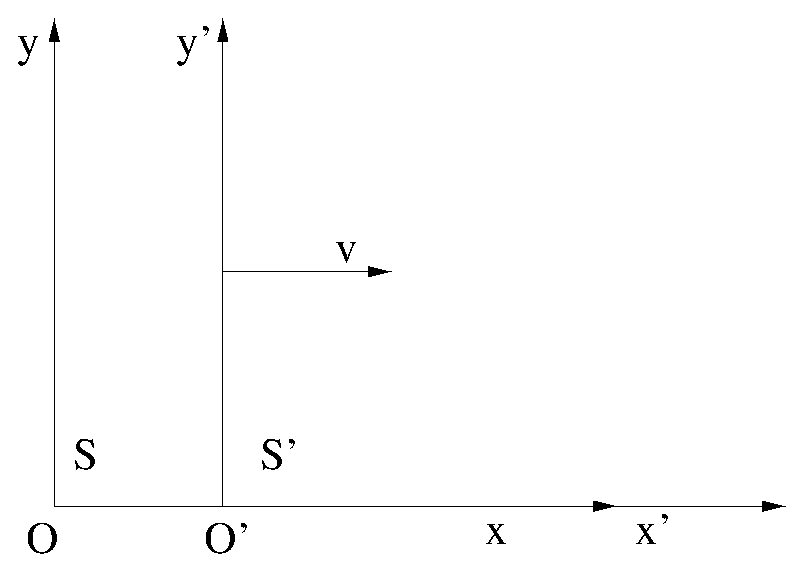
\includegraphics[width=.5\textwidth]{oefeningen.pictures/twoframes}
\caption{Twee inertiaalstelsels}
\label{f:inertiaal}
\end{figure}

Twee inertiaalstelsels $S$ en $S'$ zijn verbonden door 
de Lorentztransformatie (figuur \ref{f:inertiaal}):
\begin{eqnarray*}
      x' & = &  \gamma (x - \beta ct) \\
      y' & = &  y  \\ 
      z' & = &  z  \\ 
      ct' & = & \gamma (ct - \beta x) 
\end{eqnarray*}
en
\begin{eqnarray*}
      x & = &  \gamma (x' + \beta ct') \\
      y & = &  y'  \\
      z & = &  z'     \\
      ct & = & \gamma (ct' + \beta x')
\end{eqnarray*}

\begin{itemize}
\item [a.]
  Laat  zien  dat  de tweede set vergelijkingen (met +$\beta$) uit 
de eerste set kan worden afgeleid. 
\item [b.]
  De oorsprong van $S$ heeft $x = 0$. 
Laat met de Lorentztransformatie zien dat de oorsprong van $S$ met 
snelheid $-v$ door 
$S'$ beweegt.
\item [c.]
  Vanuit  de oorsprong van $S'$ schijnt een lichtstraal (met snelheid $c$) 
in de positieve $x'$-richting, volgens $x' = ct'$.  
Gebruik  de  Lorentztransformatie  om  aan te tonen dat hij ook een 
snelheid $c$ in $S$ heeft (dus beweegt volgens $x = ct$). 
\item [d.]
  Nu  schijnt een  lichtstraal  langs  de  $y$-as  van  $S'$  (loopt  volgens  
$y'=ct'$).  
Bepaal  met de Lorentztransformatie de totale snelheid 
$\sqrt{v^{2}_{x}+v^{2}_{y}}$ in $S$.
\end{itemize}

%%%%%%%%%
\subsection{Klokken}
$S$  en $S'$ als in figuur \ref{f:lorentz2-2}. 
Twee gebeurtenissen $A$ en $B$ die in $S$ op  dezelfde  tijd  ($t_{A}=t_{B}$)  
maar  op  verschillende  plaats  ($x_{A}\neq x_{B}$) plaatsvinden, 
zijn in $S'$ niet gelijktijdig ($t'_{A}\neq t'_{B}$).

% \begin{figure} [h]
% \begin{center}
% \mbox{\epsfxsize=8cm\epsffile{oefeningen.pictures/clocks.eps}}
% \caption{Klokken}
% \label{f:lorentz2-2}
% \end{center}
% \end{figure}
\begin{figure}[ht]
\centering
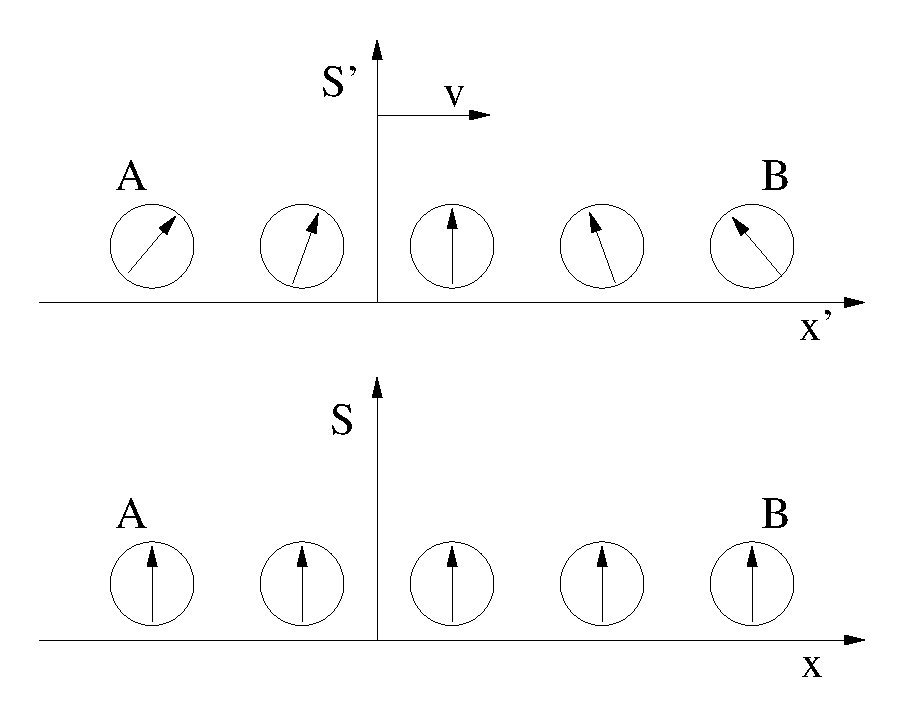
\includegraphics[width=0.8\textwidth]{oefeningen.pictures/clocks}
\caption{Klokken}
\label{f:lorentz2-2}
\end{figure}

\begin{itemize}
\item [a.]
Laat zien dat $t'_{B}-t'_{A} = -\frac{\gamma \beta}{c}(x_{B}-x_{A}$).
\item [b.]
Ga na dat figuur \ref{f:lorentz2-2}, waarin overal in 
$S$  de klokken op $t = 0$ staan, de 
klokken in $S'$ de situatie goed weer geven.
M.a.w. is het juist dat in $S'$ de klok bij $A$ v\'{o}\'{o}r loopt 
in vergelijking met de klok in $S$ en 
in $B$ achter.
\item [c.]
Geef  de  formule  voor  het  tijdsverschil $t_{B}-t_{A}$ voor 
gebeurtenissen   die   zich   in $S'$ gelijktijdig 
($t'_{A}=t'_{B}$) afspelen op $x'_{A}$ en $x'_{B}$.
\item [d.]
Teken  nu  op de manier van vraag b) de situatie voor de klokken op het 
ogenblik $t' = 0$ (de klokken in $S'$ staan nu overal op nul). 
Welke $S$-klokken lopen voor, welke achter?
\item [e.]
 Is  er  een tegenspraak tussen de figuren van vraag b) en c), 
dus zijn er b.v. passanten die van elkaar zeggen dat de klok van de 
ander voor (of achter) loopt?
\item [f.]
  Hoe  kan het dat de klokken van het andere stelsel die bij hun nadering 
nog voorliepen, achterlopen als ze gepasseerd zijn?
\end{itemize}

%%%%%%%%%%%
\subsection{Knal en lichtflits}
Op $t = 0$ klinkt een knal in $S$(figuur \ref{f:knal}).

% \begin{figure} [h]
% \begin{center}
% \mbox{\epsfxsize=8cm\epsffile{oefeningen.pictures/flash.eps}}
% \caption{Knal of lichtflits}
% \label{f:knal}
% \end{center}
% \end{figure}

\begin{figure}[ht]
\centering
\includegraphics[width=.8\textwidth]{oefeningen.pictures/flash}
\caption{Knal of lichtflits}
\label{f:knal}
\end{figure}

\begin{itemize}
\item [a.]
Bereikt  het geluid volgens een stilstaande waarnemer ($S$) $A$ eerder of 
later dan $B$? 
\item [b.]
Teken  nu  de  situatie gezien door een waarnemer die met snelheid $v$ 
naar rechts beweegt ($S'$). 
Waar komt het geluid volgens $S'$ eerder, in $A$ of in $B$? 
\end{itemize}
In plaats van een knal is er een lichtflits in $S$ op $t = 0$. 
\begin{itemize}
\item [c.]
Waar is volgens $S$ het licht eerder, in $A$ of in $B$? 
\item [d.]
Teken  de situatie volgens $S'$. 
Waar komt het licht eerder aan, in $A$ of in $B$? 
\end{itemize}

%%%%%%%%%%%%
\subsection{Boeven vangen}
%In  de situatie van de opgave `Twee inertiaalsystemen'  beweegt een 
%voorwerp met snelheid $V'$ langs de 
%$x$-as van $S'$, volgens 
%$x' = V't'$.  
%$S'$ beweegt zelf met snelheid $v$ langs de $x$-as van $S$, zodat je 
%niet-relativistisch zou verwachten dat het voorwerp met een snelheid 
%$V' + v$ door $S$ beweegt.

We bekijken een situatie, vergelijkbaar met de opgave `Twee intertiaalsystemen' uit Hoofdstuk 1, waarin we de snelheid van een voorwerp in een (voor de waarnemer in stelsel $S$) bewegend inertiaalsysteem $S'$ bekijken. In dit geval gaat het om een achtervolgingssc\`ene waarin vanuit een politie auto (stelsel $S'$) een kogel met een snelheid $v'_k$ wordt afgeschoten richting ontsnappende boeven, die een snelheid $w$ hebben in stelsel $S$.


 \begin{figure} [h]
 \begin{center}
 \mbox{\epsfxsize=14cm\epsffile{oefeningen.pictures/police2.eps}}
 \caption{Boeven vangen}
 \label{f:boeven}
 \end{center}
 \end{figure}

% plaatje veranderen (1/2 <--> 1/3) + bijschrift van snelheden
% of opdracht veranderen (1/2 <--> 1/3)

%\begin{figure}[h]
%\centering
%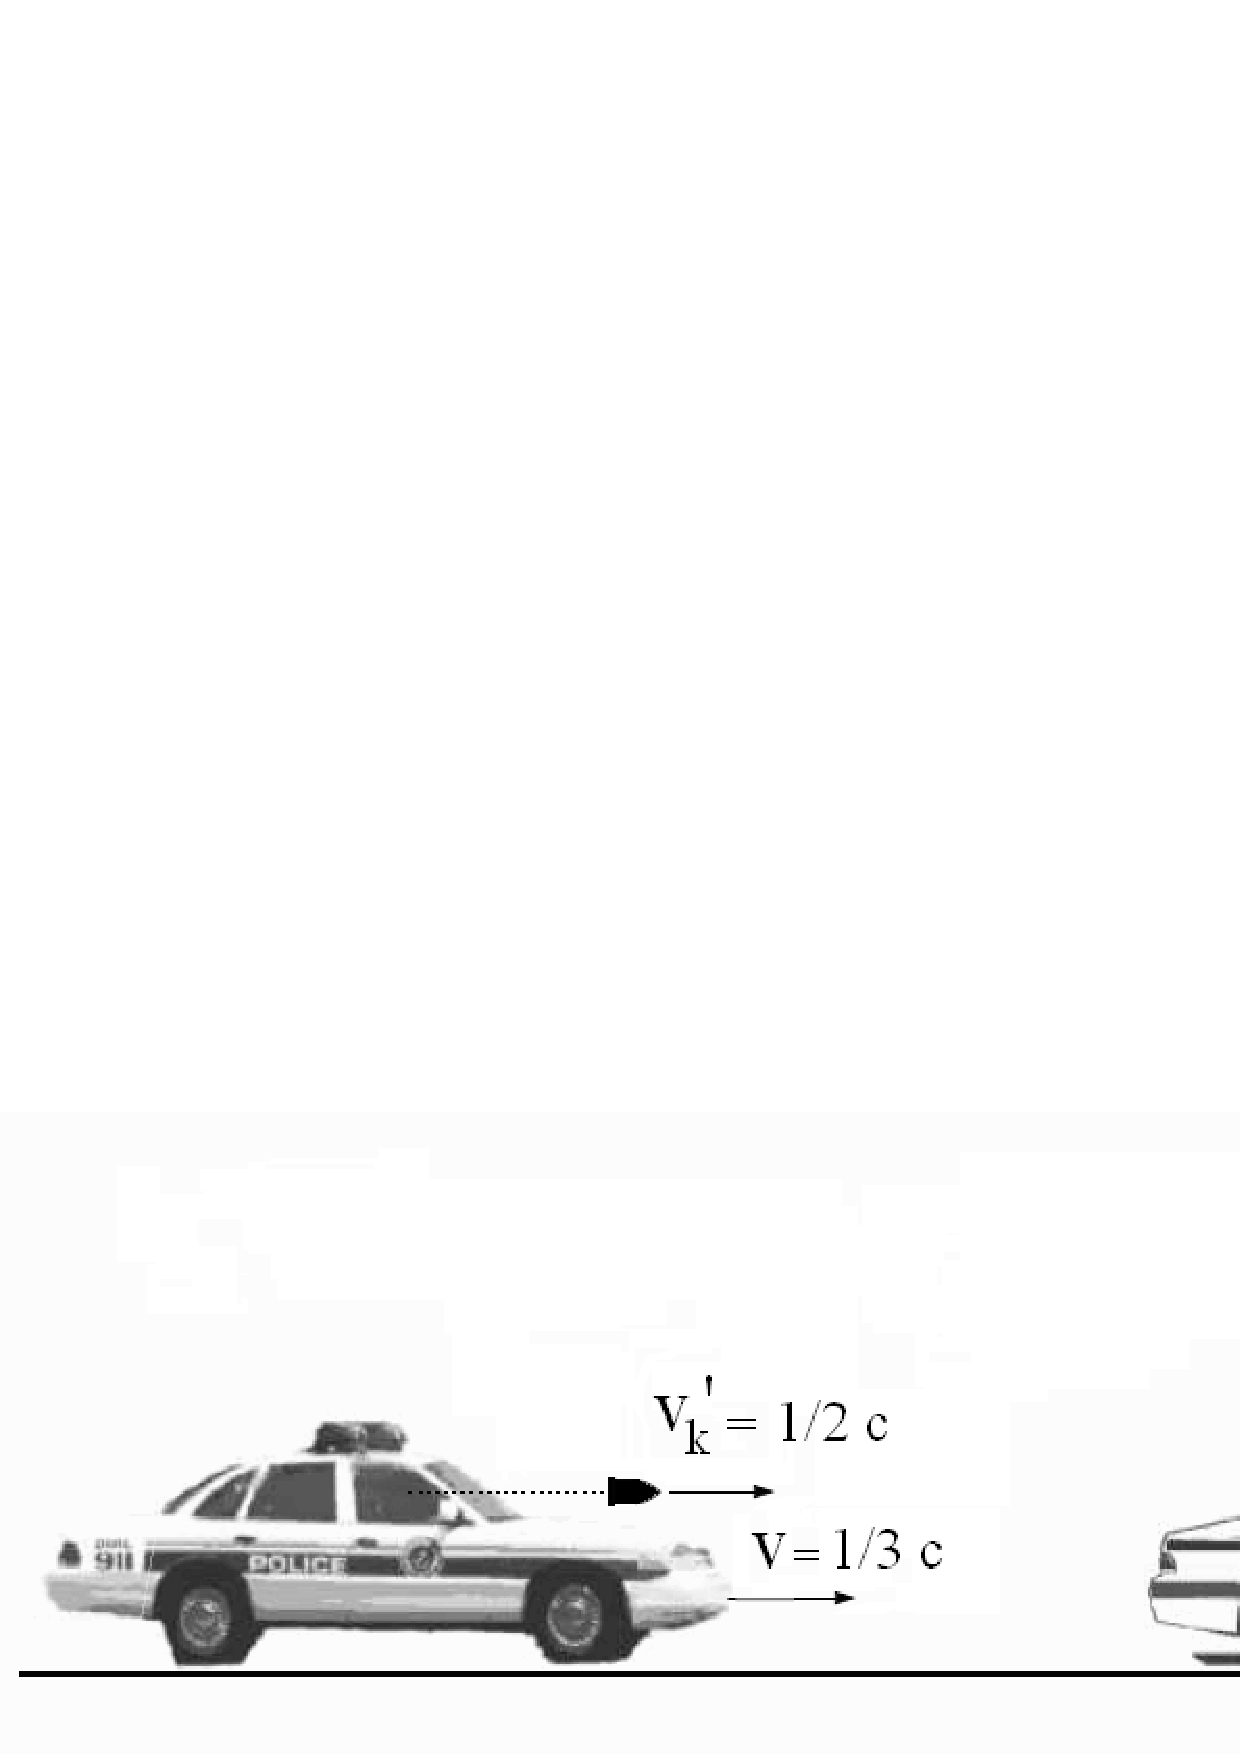
\includegraphics[width=.09\textwidth]{police2.png}
%\caption{Boeven vangen}
%\label{f:boeven}
%\end{figure}



\begin{itemize}
\item [a.]
  Vul  de  bewegingsvergelijking  $x_k' = v_k't'$ in in de formules van de 
Lorentztransformatie en leidt hieruit een verband tussen 
$x_k$ en $t$ af.
\item [b.]
  Leidt uit het resultaat van vraag a) de relativistische `optelformule voor snelheden' af: 

\begin{displaymath}
  v_k = \frac{v_k' + v}{1 + v_k'v/c^{2}}.
\end{displaymath}
\end{itemize}

De Boeven proberen met een snelheid $w =\frac{3}{4}c$ te ontkomen aan een 
achtervolgende politieauto met snelheid 
$v = \frac{1}{3}c$ (figuur \ref{f:boeven}).
De achtervolgers schieten kogels af met snelheid $v_k'=\frac{1}{2}c$.
\begin{itemize}
\item [c.]
  Volgens de gewone optelling is $\frac{1}{3} + \frac{1}{2} > \frac{3}{4}$. 
Bereken de snelheid van de kogel nu met de relativistische optelformule voor snelheden; zullen de kogels de boeven dus uiteindelijk raken?

\end{itemize}

\begin{itemize}
	\item [d.]
  Wat  geeft de optelformule als je $v_k'=c$ neemt? 
Dus: als er in plaats van een kogel met snelheid $v_k' < c$, een laserstraal (met $v_l' = c$) wordt afgevuurd richting de boeven; 
  komt het licht er dan met snelheid $c + v$ uit?
\end{itemize}


%%%%%%%%%%%%
\subsection{Raketten 1}\label{prob:rak3}

 \begin{figure} [h]
 \begin{center}
 \mbox{\epsfxsize=10cm\epsffile{oefeningen.pictures/PQ1.eps}}
 \caption{Raketten P en Q in stelsel S}
 \label{f:raktt}
 \end{center}
 \end{figure}

	
	We bekijken een situatie waarin twee raketten $P$ en $Q$ van elkaar vandaan vliegen. Op het tijdstip $t=0$ passeren de raketten elkaar boven de Aarde, dus $x_P(t=0) = x_Q(t=0) =0$ Ten opzichte van het stelsel op aarde, $S$, hebben de raketten een snelheid van respectievelijk $v_P = -\frac{4}{5} c$ en $v_Q = \frac{4}{5} c$. Het stelsel van raket $P$ noemen we $S'$.

	
		
		\begin{enumerate}
			\item[a.]
			Schrijf de Lorentz-transformatie op tussen stelsel $S$ en $S'$.
			
				\item[b.]
				Ga uit van de Lorentztransformaties en geef een uitdrukking voor de snelheid van Q gezien vanuit raket P: $v_Q'$. Controleer dat je
hiermee de `relativistische optelformule' voor snelheden terugvindt:
			
			\begin{equation}
				v'_Q = \frac{-v_P + v_Q}{1-\frac{v_P v_Q}{c^2}}
				\label{eq:1}
			\end{equation}
			
			\item[c.]
			Geef de waarde van $v'_Q$.
			
			\item[d.]
			We bepalen nu de lengte van raket $Q$ in de richting van de beweging.
			In stelsel $S$ meten we een lengte van 12 meter ($L_Q=12\,m$).\\
			Geef de lengte van $Q$ in zijn eigen ruststelsel. 
	  	
	  	\item[e.]
  		 Bereken de $(\gamma)'$-factor voor de beweging van raket $Q$ in stelsel $S'$. Wat is de lengte van raket $Q$ voor een waarnemer in raket $P$, dus ($L_Q'$)? (Je mag evt. wortels en breuken laten staan in je antwoord)
			
			\item[f.]
			 Voor een
waarnemer in $S$ verwijderen $P$ en $Q$ zich met een snelheid van 8/5 c van
elkaar. Laat aan de hand van het antwoord op vraag c. zien dat een lichtsignaal verzonden vanaf raket $P$ alsnog de waarnemer in $Q$ kan bereiken.
			\item[g.]
			Verklaar waarom de waarnemer in $S$ tevens concludeert dat dit signaal vanuit $P$ de waarnemer in $Q$ bereikt.
			
		\end{enumerate}

%%%%%%%%%%%%
\subsection{Michelson-Morley experiment}
(Analyse van het Michelson-Morley-experiment met licht)

% \begin{figure} [h]
% \begin{center}
% \mbox{\epsfxsize=10cm\epsffile{oefeningen.pictures/michelson.eps}}
% \caption{Michelson-Morley experiment}
% \label{f:mm-geluid}
% \end{center}
% \end{figure}

\begin{figure}[ht]
\centering
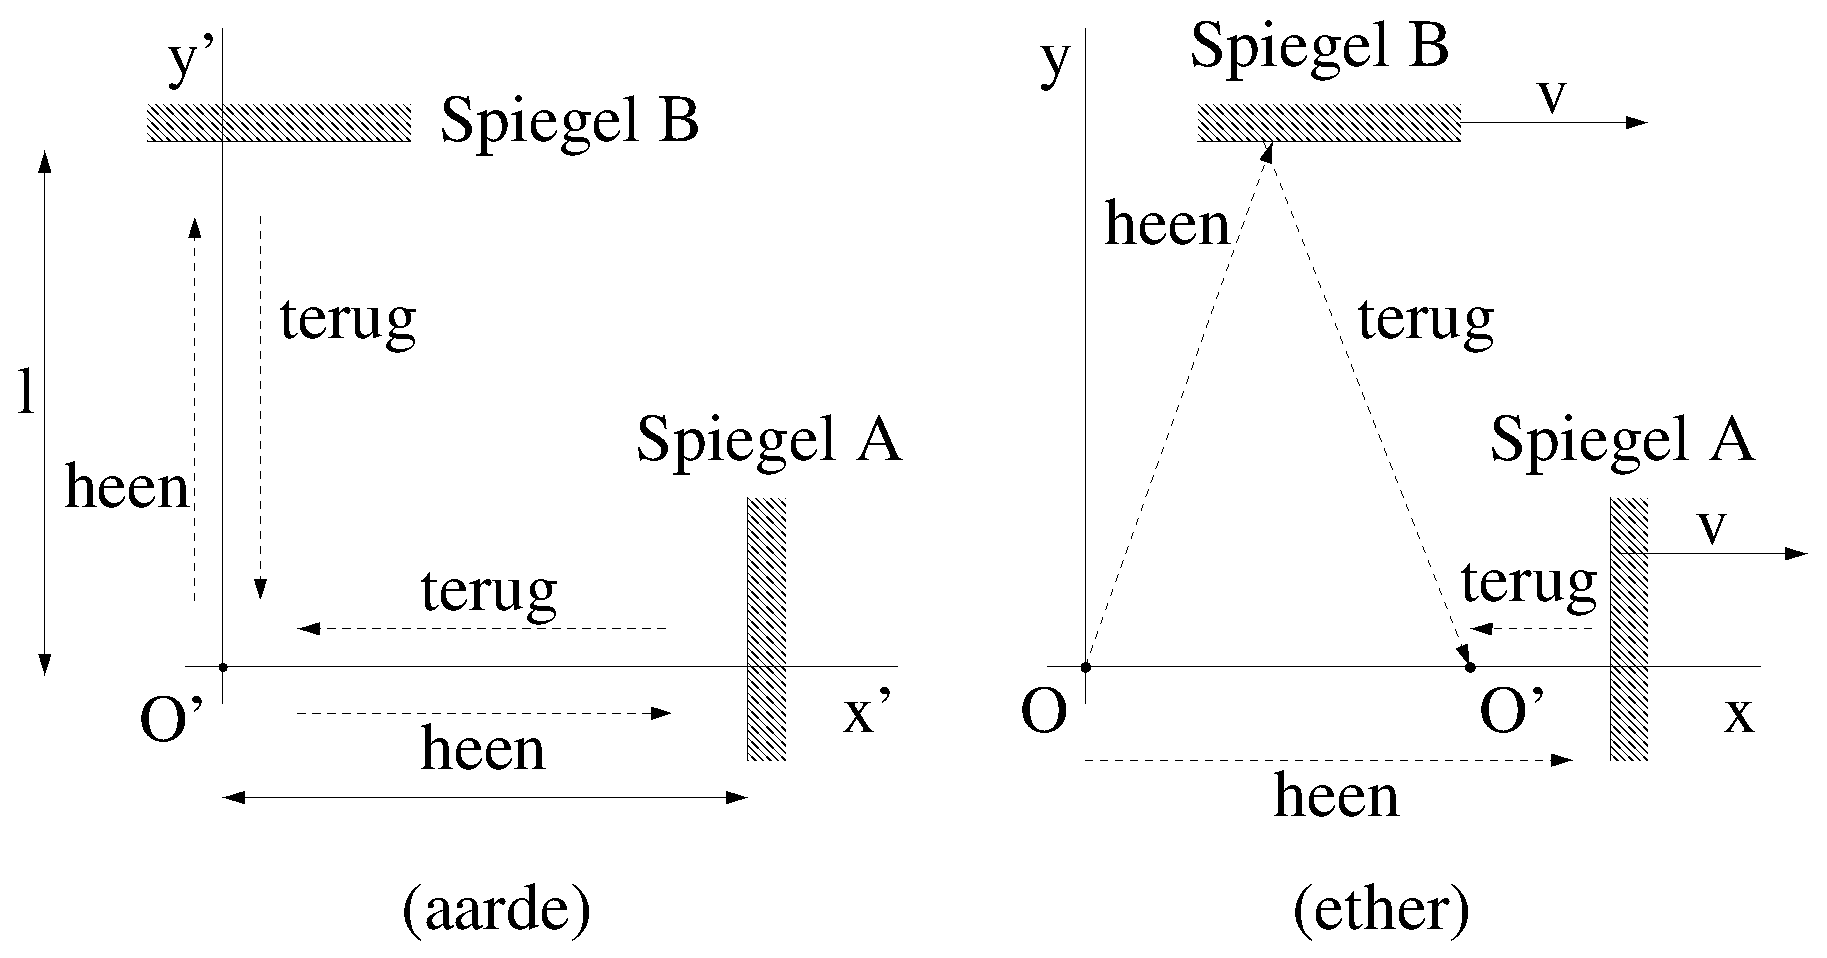
\includegraphics[width=.9\textwidth]{oefeningen.pictures/michelson}
\caption{Michelson-Morley experiment}
\label{f:mm-geluid}
\end{figure}

De aarde ($S'$) beweegt met snelheid $v$ door de `ether' ($S$).\\
In $S'$ worden lichtstralen vanuit de oorsprong $O'$ door spiegels $A$ en $B$ 
op afstand $l$ op de $x'$- en $y'$-assen teruggekaatst.\\
Omdat  we  voorlopig  alleen  weten  dat  de  lichtsnelheid  in de ether 
($S$) gelijk is aan $c$, berekenen  we  de  gebeurtenis in $S$. 
Daarna transformeren we met de Lorentztransformatie terug 
naar $S'$ en vragen ons af of er verschil in reistijd zit 
(zoals voor geluid in de opgave `Michelson-Morley voor geluid').

De  beweging  $O'AO'$  langs  de  $x'$-as ziet er in $S$ uit als links in 
figuur \ref{f:mm-geluid}: 
de heenreis  duurt  $t_{h}$,  met  een  snelheid  $c$  over  een  afstand 
$\gamma ^{-1}l+vt_{h}$ (want door de 
Lorentzcontractie  is  de  lengte  $\gamma ^{-1}l$  en  is de
spiegel  $A$  naar rechts verschoven met snelheid $v$).
De terugreis  duurt  $t_{t}$,  met  een  snelheid $c$, over een afstand 
$\gamma ^{-1} l-vt_{t}$ (want de oorsprong $O'$ is 
dichterbij gekomen met snelheid $v$).

\begin{itemize}
\item [a.]
  Laat zien dat de beweging $O'AO'$ volgens $S$ een tijd 
\begin{displaymath}
  t_{x} \equiv t_{h} + t_{t} = \frac{2 \gamma l}{c}
\end{displaymath}
geduurd heeft en dat $O'$ dan zit op 
\begin{displaymath}
x = 2 \gamma \beta l
\end{displaymath}
\end{itemize}

De beweging $O'BO'$ langs de $y'$-as ziet er in $S$ uit als rechts in
Figuur ~\ref{f:mm-geluid}.
Heen-  en terugreis  duren  even lang en  overbruggen met 
een snelheid $c$ een afstand $\sqrt{l^{2} + (vt)^{2}}$
(want spiegel $B$ is naar rechts verschoven met snelheid $v$).

\begin{itemize}
\item [b.]
Waarom heeft de lat nu geen Lorentz-contractie?
\item [c.]
Laat zien dat de beweging $O'BO'$ volgens $S$ een tijd
\begin{displaymath}
t_{y} \equiv t_{h} + t_{t} = \frac{2 \gamma l}{c}
\end{displaymath}
geduurd heeft.
\end{itemize}
De  lichtstralen  keren  dus in $S$ tegelijkertijd terug.
De vraag was echter of je op aarde, in $S'$, verschil in terugkeertijd ziet.

\begin{itemize}
\item [d.]
Zijn de twee reistijden na 
Lorentztransformatie van $S$ naar $S'$ ook hetzelfde?
\item [e.]
Wat is de conclusie met betrekking tot het bestaan van de `ether'?
\end{itemize}

